\documentclass[25pt, a0paper, landscape, margin=0mm, innermargin=18mm, blockverticalspace=14mm, colspace=16mm]{tikzposter}
% Poster for the CS 5180 project; figure and tables are the report's (report/paper/main.tex),
% numbers from report/phase7/prereg_analysis.json.
\usepackage[T1]{fontenc}
\usepackage{mathptmx}
\usepackage{booktabs}
\usepackage{graphicx}
\usepackage{amsmath,amssymb}

\definecolor{ink}{HTML}{1F1F1E}
\definecolor{muted}{HTML}{6B6A64}
\definecolor{bcblue}{HTML}{2A78D6}
\definecolor{iqlorange}{HTML}{EB6834}
\definecolor{surface}{HTML}{FCFCFB}
\definecolor{band}{HTML}{EFEEEA}

\definecolorstyle{plain}{}{
  \colorlet{backgroundcolor}{surface}
  \colorlet{framecolor}{band}
  \colorlet{titlefgcolor}{ink}
  \colorlet{titlebgcolor}{surface}
  \colorlet{blocktitlebgcolor}{surface}
  \colorlet{blocktitlefgcolor}{ink}
  \colorlet{blockbodybgcolor}{surface}
  \colorlet{blockbodyfgcolor}{ink}
  \colorlet{innerblocktitlebgcolor}{band}
  \colorlet{innerblocktitlefgcolor}{ink}
  \colorlet{innerblockbodybgcolor}{band}
  \colorlet{innerblockbodyfgcolor}{ink}
  \colorlet{notefgcolor}{ink}
  \colorlet{notebgcolor}{band}
  \colorlet{notefrcolor}{band}
}
\usecolorstyle{plain}
\usetitlestyle{Empty}
\useblockstyle{Minimal}
\usebackgroundstyle{Empty}

\title{\parbox{0.9\linewidth}{\centering How Much Expert Data Does Offline RL Need?\\[0.25em]
\normalsize\Large Behavior Cloning vs.\ Implicit Q-Learning on Mixed-Quality Hopper Datasets}}
\author{Rahul Vishnuvardhana \quad Khoury College of Computer Sciences, Northeastern University \quad CS 5180 Reinforcement Learning}
\institute{}

\newcommand{\Ps}{P}
\tikzposterlatexaffectionproofoff
\begin{document}
\maketitle[width=0.95\linewidth]

\begin{columns}
\column{0.25}
\block{Question}{
Real logs mix good and poor behavior. We make the \textbf{fraction of expert data} $p$ the independent variable and ask how quickly \textcolor{bcblue}{\textbf{behavior cloning (BC)}} and \textcolor{iqlorange}{\textbf{Implicit Q-Learning (IQL)}} reach expert performance as it grows.

\vspace{0.6em}
\textbf{Hypotheses} (pre-registered 2026-11-21, before any grid result)
\begin{itemize}
  \item \textbf{H1} BC's score rises with $p$, possibly non-monotonically.
  \item \textbf{H2} IQL reaches near-expert ($\geq 90$) at a much lower $p$ than BC.
  \item \textbf{H3} A higher expectile $\tau$ helps IQL more at $p=0.05$ than at $p=0.5$.
\end{itemize}
}
\block{Setup}{
\begin{itemize}
  \item Hopper-v5 (MuJoCo); Minari \texttt{expert-v0} and \texttt{simple-v0}.
  \item Mixtures of 900k transitions, $p\in\{0, 0.05, 0.2, 0.5, 1\}$, whole episodes.
  \item Same Gaussian policy, buffer, normalization and budget for both; BC is IQL's policy loss with $\beta=0$.
  \item IQL $\tau=0.7$; ablation $\tau\in\{0.5, 0.9\}$ at $p\in\{0.05, 0.5\}$.
  \item 5 seeds, 300k steps: \textbf{70 runs}, one commit, one CPU type, 3.1 h wall clock.
  \item Score: 0 = random policy, 100 = expert data mean; last 5 evaluations $\times$ 50 episodes.
  \item Tests: exact one-sided paired sign-flip over 5 seeds (level 0.05, smallest $P=1/32$). \textbf{No correction across H1 to H3.}
\end{itemize}
}

\column{0.50}
\block{Results}{
\centering
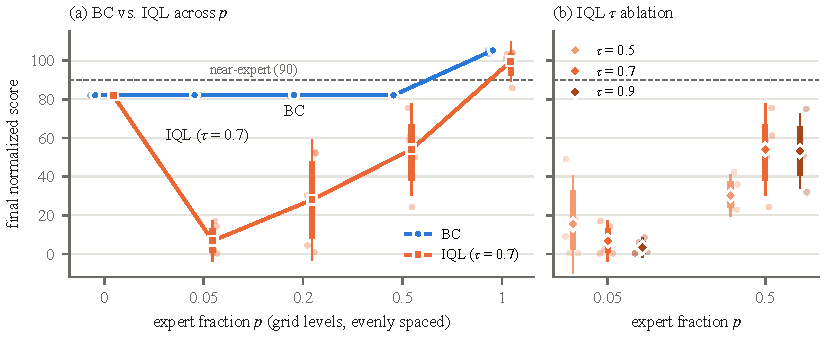
\includegraphics[width=0.98\linewidth]{../figures/score_vs_p.pdf}

\vspace{0.3em}
{\small Dots: seeds; markers: mean; thin whisker: 95\% t-interval; thick bar: 95\% bootstrap interval; dashed: near-expert (90).}

\vspace{0.8em}
\begin{tabular}{@{}lllr@{\hspace{0.8em}}l@{}}
  \toprule
  & Pre-registered test (one-sided) & Per seed & $\bar d$ & Verdict \\
  \midrule
  H1 & BC($p{=}1$) $-$ BC($p{=}0$) & 23.2, 21.3, 24.1, 23.0, 24.4 & $+23.2$ & \textbf{Supported} ($P=0.031$) \\
  H2 & IQL $-$ BC at $p=1$ (both cross only there) & $-4.4, -0.1, -2.2, -19.4, -2.3$ & $-5.7$ & \textbf{Not supported} ($P=1.000$) \\
  H3 & $\tau$ effect at $p{=}0.05$ minus at $p{=}0.5$ & $-61.6, -22.6, -57.2, -38.2, +4.6$ & $-35.0$ & \textbf{Inconclusive} ($P=0.969$) \\
  \bottomrule
\end{tabular}
}
\block{IQL's collapse comes with falls}{
\begin{itemize}
  \item Pre-registered flags: \emph{high-fall} if a run falls in at least half of its 250 final episodes, \emph{collapsed} if it scores below 10. Flagged runs stay in every statistic.
  \item At $p=0.05$ every IQL run is high-fall (cell fall rates 0.88 to 1.00) and 11 of its 15 runs (all three $\tau$) collapsed.
  \item BC never falls below $p=1$; at $p=0$ (simple data only) IQL is stable too (fall rate 0.02).
  \item Why IQL becomes unstable with scarce expert data was not tested; one candidate is advantage weighting concentrating the policy on few expert transitions.
\end{itemize}
}

\column{0.25}
\block{Final scores (mean of 5 seeds)}{
\centering
\begin{tabular}{@{}lrrrrrr@{}}
  \toprule
  $p$ & 0 & 0.05 & 0.2 & 0.5 & 1 \\
  \midrule
  \textcolor{bcblue}{\textbf{BC}} & 82.2 & 82.2 & 82.2 & 82.1 & 105.4 \\
  \quad fall rate & 0.00 & 0.00 & 0.00 & 0.00 & 0.03 \\
  \textcolor{iqlorange}{\textbf{IQL}} $\tau{=}0.7$ & 82.0 & 6.7 & 28.0 & 54.1 & 99.7 \\
  \quad fall rate & 0.02 & 0.98 & 0.77 & 0.61 & 0.10 \\
  \midrule
  IQL $\tau{=}0.5$ & & 15.3 & & 30.2 & \\
  IQL $\tau{=}0.9$ & & 3.2 & & 53.1 & \\
  \bottomrule
\end{tabular}

\vspace{0.4em}
\raggedright
\textit{Exploratory tests (comparisons pre-registered as descriptive only), uncorrected:} BC leads IQL on all 5 seeds at $p=0.05$, $0.2$, $0.5$ and $1$ (each $P=0.031$).
}
\block{Demo: median seeds at $p=0.05$}{
\centering
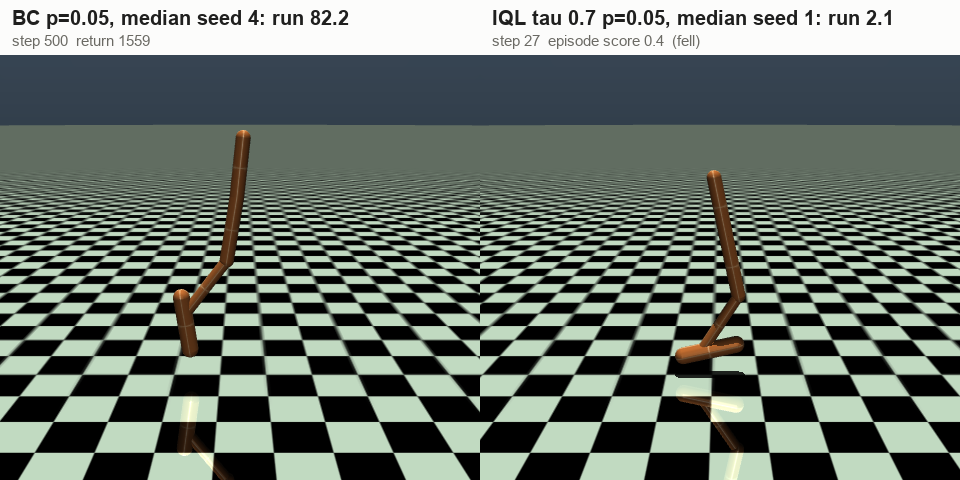
\includegraphics[width=\linewidth]{demo_frame.png}

\vspace{0.3em}
\raggedright\small
Evaluation seed 10000, each cell's median-scoring run, final policies (300k). The episodes match the logged evaluation exactly: BC hops for all 1000 steps; IQL falls after 27. Frame at 4 s of the video (\texttt{scripts/record\_demo.py}, \texttt{--frame-at 4}).
}
\block{Takeaway}{
\begin{itemize}
  \item BC gains nothing from expert data up to $p=0.5$, then reaches 105 at $p=1$ (no $p$ between 0.5 and 1 run).
  \item IQL does not match BC at any $p>0$ (it trails by 5.7 even at $p=1$); with scarce expert data it falls (98\% of episodes at $p=0.05$).
  \item Limits: 5 seeds (low power), one environment and dataset pair, untuned $\beta$; CORL check shared our preprocessing; two IQL cells still climbing at 300k.
\end{itemize}

{\small References: IQL (Kostrikov et al., ICLR 2022); Minari (Farama, 2024); CORL (Tarasov et al., 2023); MuJoCo; Gymnasium.}
}
\end{columns}

\end{document}
